\documentclass[
%a4paper,12pt
encoding=utf8
]{../twoeskd}

% \usepackage{eskdappsheet}

% Packages required by doxygen
\usepackage[export]{adjustbox} % also loads graphicx
\usepackage[draft]{graphicx}
\usepackage[utf8]{inputenc}
\usepackage{multicol}
\usepackage{multirow}
\usepackage{makeidx}

% NLS support packages
\usepackage[T2A]{fontenc}
\usepackage[russian]{babel}
\usepackage{pscyr}

% Font selection
\usepackage{courier}
\usepackage{amssymb}

% Page & text layout
% \usepackage{geometry}
% \geometry{%
%   a4paper,%
%   top=2.5cm,%
%   bottom=4.5cm,%
%   left=2.5cm,%
%   right=2.5cm%
% }
%\setlength{\emergencystretch}{15pt}
\setlength{\parindent}{0cm}
\setlength{\parskip}{0.2cm}

% Headers & footers
% \usepackage{fancyhdr}
% \pagestyle{fancyplain}
% \fancyhead[L]{\fancyplain{}{}}
% \fancyhead[C]{\fancyplain{}{\scriptsize\textbf{RU.17701729.509000 ТЗ 01-1-ЛУ}}}
% \fancyhead[R]{\fancyplain{}{}}
% \fancyfoot[L]{\fancyplain{}{}}
% \fancyfoot[C]{\fancyplain{}{}}
% \fancyfoot[R]{\fancyplain{}{}}

% debug to see the frame borders
% from https://en.wikibooks.org/wiki/LaTeX/Page_Layout
% \usepackage{showframe}

% Indices & bibliography
\usepackage{natbib}
\usepackage[titles]{tocloft}
\setcounter{tocdepth}{3}
\setcounter{secnumdepth}{5}
\makeindex

% change style of titles in \section{}
\usepackage{titlesec}
\titleformat{\section}[hang]{\huge\bfseries\center}{\thetitle.}{1em}{}
\titleformat{\subsection}[hang]{\Large\normalfont\raggedright}{\thetitle.}{1em}{\underline}
\titleformat{\subsubsection}[hang]{\large\normalfont\raggedright}{\thetitle.}{1pt}{}

% Packages for text layout in normal mode
% \usepackage[parfill]{parskip} % автоматом делает пустые линии между параграфами, там где они есть в тексте
% \usepackage{indentfirst} % indent even in first paragraph
\usepackage{setspace}	 % controls space between lines
\setstretch{1} % space between lines
\setlength\parindent{0.9cm} % size of indent for every paragraph
\usepackage{csquotes}% превратить " " в красивые двойные кавычки
\MakeOuterQuote{"}


% this makes items spacing single-spaced in enumerations.
\newenvironment{my_enumerate}{
\begin{enumerate}
  \setlength{\itemsep}{1pt}
  \setlength{\parskip}{0pt}
  \setlength{\parsep}{0pt}}{\end{enumerate}
}


% Custom commands
% configure eskd
\titleTop{
\textbf{\Large ПРАВИТЕЛЬСТВО РОССИЙСКОЙ ФЕДЕРАЦИИ \\
НАЦИОНАЛЬНЫЙ ИССЛЕДОВАТЕЛЬСКИЙ УНИВЕРСИТЕТ \\
«ВЫСШАЯ ШКОЛА ЭКОНОМИКИ» } \\
\vspace*{0.2cm}
{\small Факультет компьютерных наук \\
Департамент программнoй инженерии \\
}
}
\titleDesignedBy{Студент группы БПИ 151 НИУ ВШЭ}{Абрамов А.M.}
\titleAgreedBy{%
\parbox[t]{7cm} {
Профессор департамента \\
программной инженерии \\
факультета компьютерных наук \\
канд. техн. наук \\
}}{Гринкруг Е. М.}
\titleApprovedBy{
\parbox[t]{10cm} {
Академический руководитель \\
образовательной программы \\
«Программная инженерия» \\
профессор департамента программной \\
инженерии канд. техн. наук \\
}}{Шилов В. В.}
\titleName{ПРОГРАММАТОР МИКРОКОНТРОЛЛЕРОВ PIC НА ОСНОВЕ ORANGE PI LITE}
\workTypeId{RU.17701729.509000 34 01-1}

\titleSubname{Руководство оператора}

% Custom packages
\usepackage{pdfpages}

\makeindex

%===== C O N T E N T S =====


\begin{document}
% Titlepage & ToC
\pagenumbering{roman}

% some water filling text, that is pointless but adds text
% \input{annotation}

\newpage
\pagenumbering{arabic}
\tableofcontents
% \pagenumbering{arabic}

% --- add my custom headers ---
\newpage
\section{Назначение программы}
\subsection{Наименование}
Наименование: «Программатор микроконтроллеров PIC на основе Orange PI Lite». \\
Наименование на английском: «Programmer for PIC Microcontrollers Based on Orange PI Lite». \\

\subsection{Область применения}
Программа и электронная схема предназначена для работы на тонком кленте Orange Pi Lite с операционной системой семейства Linux. Программа и схема могут использоваться в учебных целях для демонстации основных компонентов необходимых для прошивки микроконтроллера. Они предоставляют новое направление использования тонкого клиента Orange Pi Lite. Ими может воспользоваться любой человек, желающий запрограммировать микроконтроллер, не имеющий на руках официального программатора, но у которого есть Orange Pi Lite. Данная программа и электронаня схема могут использоваться в качестве дешевой, простой и быстрой алтернативы к покупке официального программатора.

\newpage
\section{Условия использования программы}
%=========================================
\subsection{Минимальные параметры технических средств}
Для оптимальной работы приложения необходимо учесть следующие системные требования:
\begin{my_enumerate}
\item Тонкий клиент Orange Pi Lite, оснащенный:
    \begin{my_enumerate}
    \item Обязательно процессор Allwinner H3 с тактовой частотой 1 гигагерц (ГГц) или выше;
    \item 0.5 ГБ оперативной памяти (ОЗУ);
    \item 0.5 ГБ свободного места на жестком диске;
    \item Периферия: выход GPIO типа Rasberry Pi B+
    \end{my_enumerate}
\item Опционально: Компьютер для удаленного доступа к Orange Pi Lite, оснащенный:
    \begin{my_enumerate}
    \item Обязательно 64-разрядный (x64) процессор с тактовой частотой 1 гигагерц (ГГц) или выше;
    \item 1 ГБ оперативной памяти (ОЗУ);
    \item 1.5 ГБ свободного места на жестком диске;
    \item Wifi модулем (если Orange Pi Lite подключен к сети, то можно воспользоваться и стандартным Ethernet портом) или TTL переходником для подключения к тонкому клиенту Orange Pi Lite.
    \end{my_enumerate}
\item Монитор
\item Мышь
\item Клавиатура
\end{my_enumerate}


%=========================================
\subsection{Минимальные программные средства}
Исходный код программы для контролирования программатора обязательно должен быть написан с использованием языка C. Приложению необходим тонкий клиент с операционной системой производной от Debian с версией ядра не ниже 3.1. Приложение можно запускать как с  самого Orange Pi Lite, так и с компьютера имеющего удаленный доступ к Orange Pi Lite. В данном случае на удаленном компьютере и на тонком клиенте должны быть установленны программы для настроек удаленного доступа (например SSH, VNC viewer, TTY serial console). Для данных програм подходит любой дистрибутив Linux или 64-битная операционная система Windows 7 или более поздняя версия Windows.


\subsection{Численность и калификация персонала}
Минимальное количество персонала, требуемого для работы программы: 1 оператор. Пользователь программы должен иметь образование не ниже среднего, обладать практическими навыками работы с компьютером и электронникой.


\newpage
\section{Выполнение программы}
\subsection{Загрузка файлов}
Для загрузки данных из формата коллада (collada или .dae) необходимо выбрать его либо в меню "Open Recent", либо в меню "Open":

\begin{figure}[h!]
    \centering
    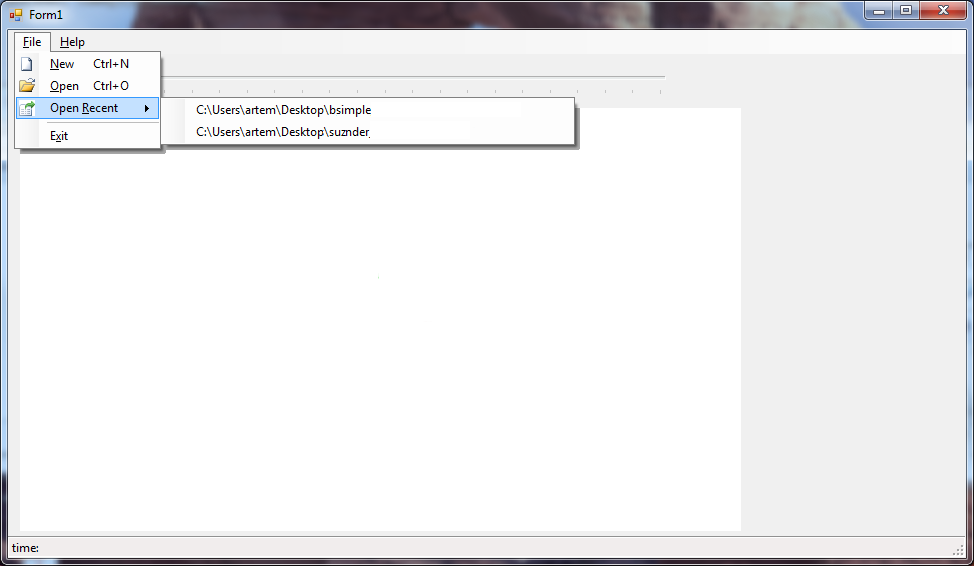
\includegraphics[width=0.8\textwidth]{../screenshots/file_menu_with_recent.png}
    \caption{Загрузка файла}
\end{figure}

Откроется диалог выбора файла:
\begin{figure}[h!]
    \centering
    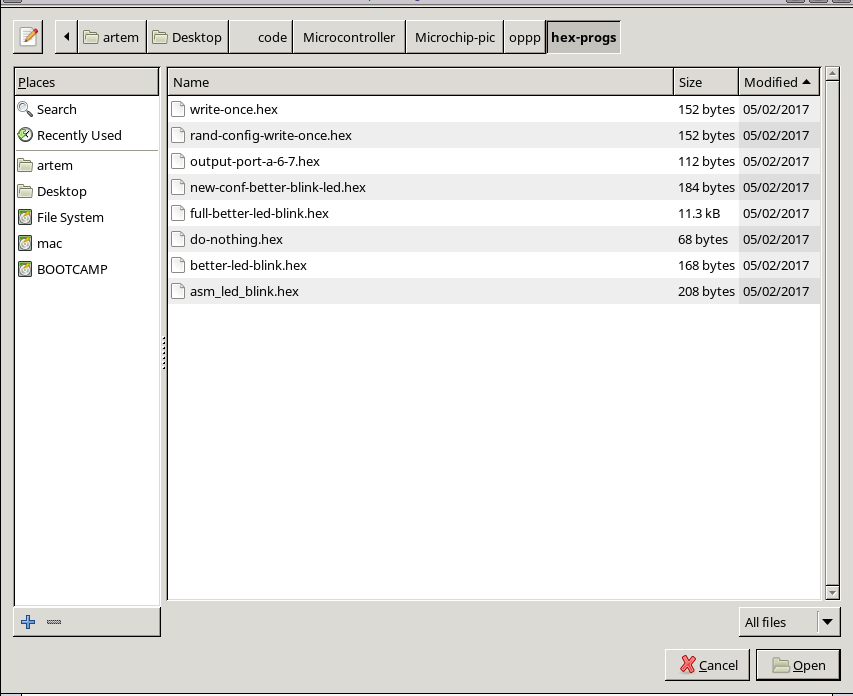
\includegraphics[width=0.5\textwidth]{../screenshots/open_file_dialog.png}
    \caption{Диалог выбора файла}
\end{figure}

После загрузки файла, его имя будет добавиленно в список недавно открытых файлов "Recent Files".

\subsection{Изменение положения камеры}
Изменять ракурс и приближение камеры можно при помощи мышки. Для приближения/отдаления используется колесо мышки. С помощью клавиш W,A,S,D можно двигать объект вверх, вправо, влево или вниз.

\subsection{Просмотр иерархии костей}
Структура загруженных данных отображена в виде дерева на панели справа. Выделенная на данный момент кость подсвеченна ярко-синим цветом.

\begin{figure}[h!]
    \centering
    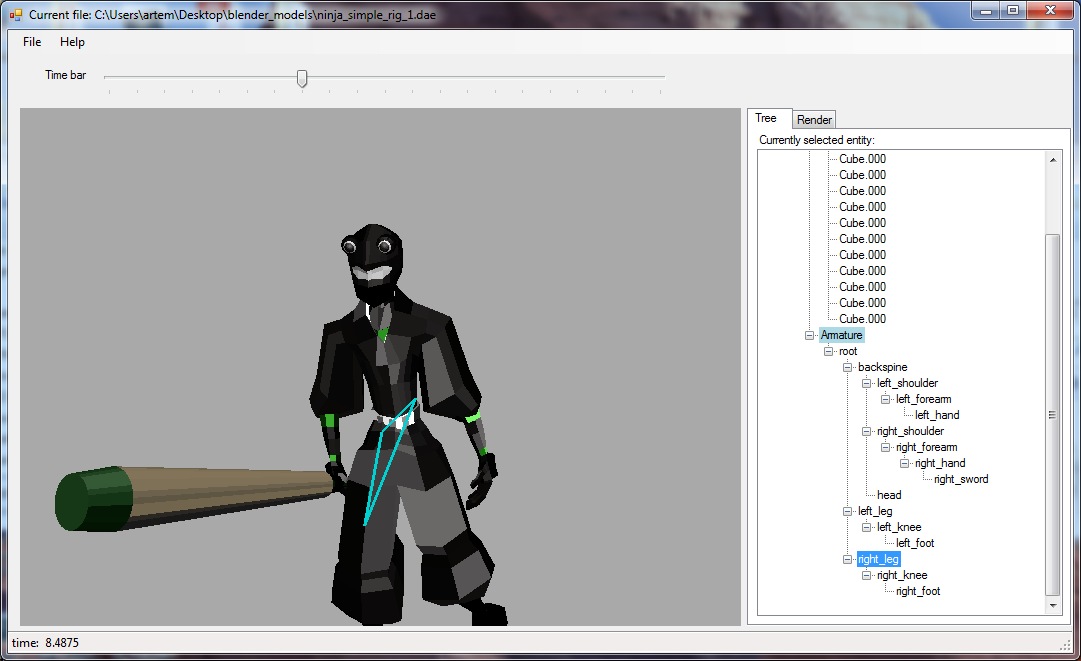
\includegraphics[width=0.8\textwidth]{../screenshots/frame_with_one_bone.png}
    \caption{Подсветка выбранной кости}
\end{figure}


\subsection{Изменение параметров отрисовки и анимации}
Элемент ScrollBar показывает текущий момент в анимации и предоставляет 
возможность перейти к любому моменту времени. 

\begin{figure}[h!]
    \centering
    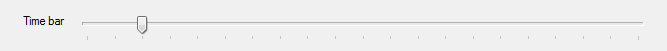
\includegraphics[width=0.5\textwidth]{../screenshots/time_bar.png}
    \caption{Элемент ScrollBar}
\end{figure}

Также есть панель для настоек работы программы позволяющая изменять следующие параметры:
\begin{my_enumerate}
\item Выбор между двумя видами камер в OpenGL, первый вид это камера движение которой сковано орбитой вокруг модели и другой тип это камера двигающаяся совершенно свободно.
\item Воспроизведение анимации.
\item Включение и выключение отрисовки с учетом нормалей.
\item Включение и выключение отрисовки с учетом характеристик материала.
\item Отрисовка всех костей скелета.
\end{my_enumerate}


\begin{figure}[h!]
    \centering
    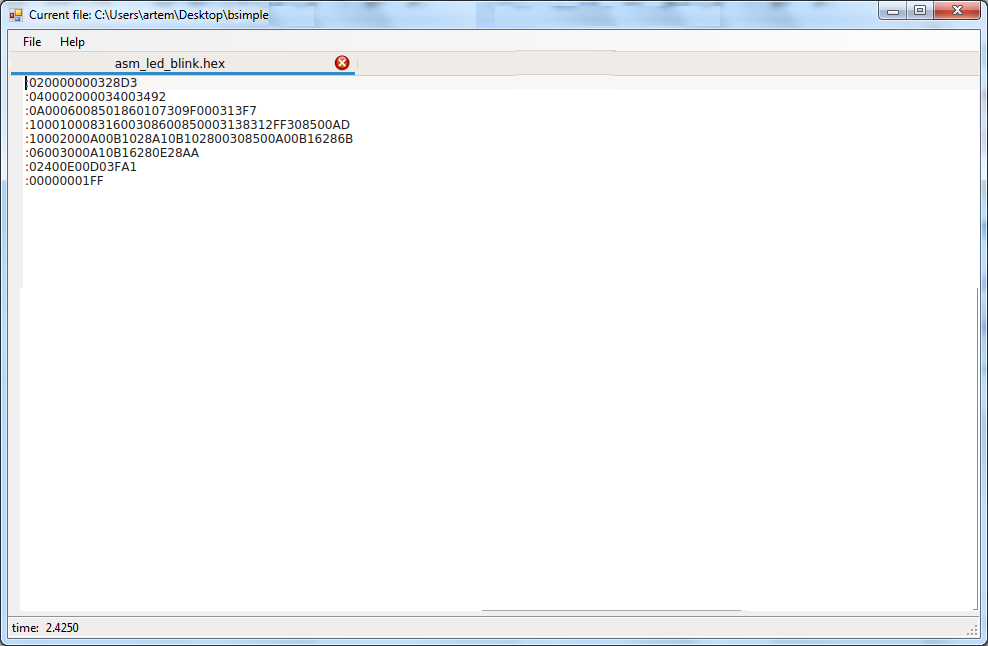
\includegraphics[width=0.8\textwidth]{../screenshots/interface_map.png}
    \caption{Справа: панель настойки отрисовки}
\end{figure}


\subsection{Всплывающие окна}
В случае если выбран файл не соответствующий требованиям входных данных отображается всплывающее окно:

\begin{figure}[h!]
    \centering
    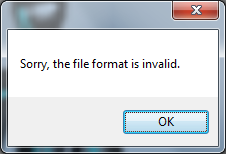
\includegraphics[width=0.3\textwidth]{../screenshots/error_message.png}
    \caption{Всплывающее окно}
\end{figure}


\subsection{Завершение работы с программой}
Происходит при нажатии на кнопку "Закрыть" в правом верхнем углу программы.


\newpage
\section{Приложение 1. Терминология}
\subsection{Терминология}
\begin{description}

\item[Корневая вершина (англ. root node)]  
Самый верхний узел дерева.

\item[Полигональная сетка (жарг. меш от англ. polygon mesh)]
Совокупность вершин, рёбер и граней, которые определяют форму многогранного объекта в трехмерной компьютерной графике и объёмном моделировании. Гранями являются треугольники.

\item[Дерево]
Связный ациклический граф. Связность означает наличие путей между любой парой вершин, ацикличность — отсутствие циклов и то, что между парами вершин имеется только по одному пути.

\item[Степень вершины]
Количество инцидентных ей (входящих/исходящих из нее) ребер.

\item[Интерполяция, интерполирование анимации]
Способ нахождения промежуточных значений состояния анимации по имеющемуся дискретному набору известных значений.

\item[Z-буферизация]
В компьютерной трёхмерной графике способ учёта удалённости элемента изображения. Представляет собой один из вариантов решения «проблемы видимости»

\item[Z-конфликт (англ. Z–fighting)]
Если два объекта имеют близкую Z-координату, иногда, в зависимости от точки обзора, показывается то один, то другой, то оба полосатым узором.

\item[OpenGL (Open Graphics Library)]
Спецификация, определяющая независимый от языка программирования платформонезависимый программный интерфейс для написания приложений, использующих двумерную и трёхмерную компьютерную графику. На платформе Windows конкурирует с Direct3D.

\item[Рендеринг (англ. rendering — «визуализация»)]
Термин в компьютерной графике, обозначающий процесс получения изображения по модели с помощью компьютерной программы.

\item[Текстура]
Растровое изображение, накладываемое на поверхность полигональной модели для придания ей цвета, окраски или иллюзии рельефа. Приблизительно использование текстур можно легко представить как рисунок на поверхности скульптурного изображения.

\end{description}



\newpage
\section{Приложение 2. Список используемой литературы}
\subsection{Список используемой литературы}
\begin{my_enumerate}
\item
ГОСТ 19.101-77 Виды программ и программных документов
//Единая система программной документации. -М.: ИПК Издательство стандартов, 2.: 001.

\item
ГОСТ 19.103-77 Обозначения программ и программных документов. //Единая система программной документации. -М.: ИПК Издательство стандартов, 2001.

\item
ГОСТ 19.104-78 Основные надписи //Единая система программной документации. -М.: ИПК Издательство стандартов, 2001.

\item 
ГОСТ 19.105-78 Общие требования к программным документам. //Единая система
программной документации. – М.: ИПК Издательство стандартов, 2001.

\end{my_enumerate}



% \newpage
%\section{Приложение 3. Изображение пользовательского интерфейса.}

% Index
\newpage
\eskdListOfChanges

% \phantomsection
% \addcontentsline{toc}{section}{Алфавитный указатель}
% \printindex

\end{document}
